\documentclass[tikz]{standalone}
\usetikzlibrary{arrows, positioning}
\tikzset{
  treenode/.style = {align=center, inner sep=1pt, text centered,
    font=\sffamily},
  arn_b/.style = {treenode, circle, white, font=\sffamily\bfseries, draw=black,
    fill=black, text width=2em},% arbre rouge noir, noeud noir
  arn_r/.style = {treenode, circle, red, draw=red, 
    text width=2em, very thick}% arbre 
}

\begin{document}
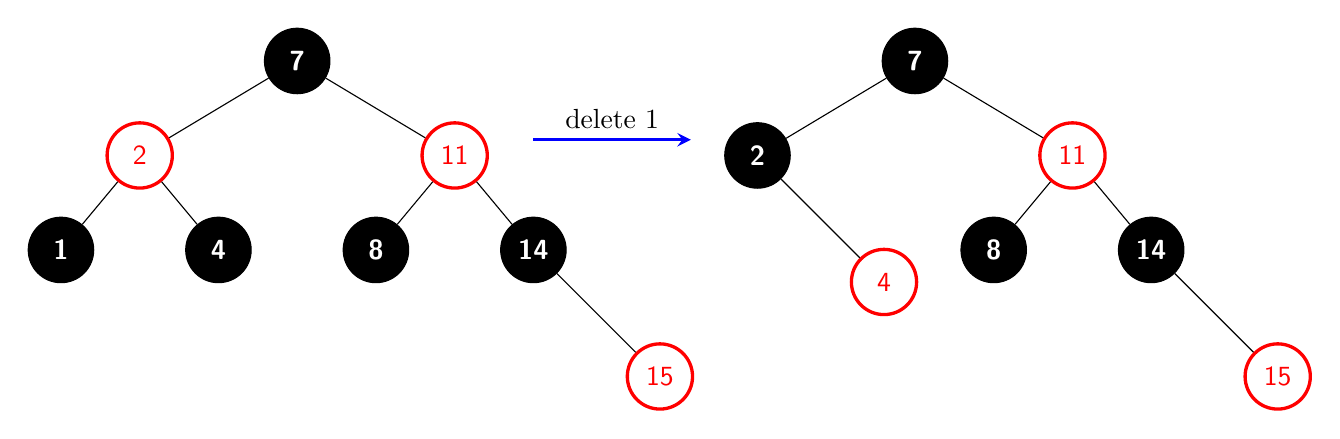
\begin{tikzpicture}[level/.style={sibling distance = 4cm/#1,
    level distance = 1.2cm}]

    \node (midtree) [arn_b] {7}
    child{node [arn_r] {2}
        child {node [arn_b] {1}}
        child {node (2n4) [arn_b] {4}
        }
        }
    child {node [arn_r] {11}
        child {node [arn_b]{8}}
        child {node (2n14) [arn_b]{14}
            child {node [arn_r, below right=of 2n14] {15}}}
    }
;

\draw [-stealth, line width=0.4mm, draw=blue](3,-1) -- (5,-1)node[midway,above,shape=rectangle,draw=none]{delete 1};

    \node (righttree) [arn_b, right=of midtree, xshift=6cm] {7}
    child{node (3n2) [arn_b] {2}
        child {node [arn_r, below right=of 3n2] {4}
        }
        }
    child {node [arn_r] {11}
        child {node [arn_b]{8}}
        child {node (3n14) [arn_b]{14}
            child {node [arn_r, below right=of 3n14] {15}}}
    }
;

\end{tikzpicture}
\end{document}